\documentclass[11pt,letterpaper]{article}
\usepackage[utf8]{inputenc}
\usepackage[spanish,USenglish]{babel}
\usepackage{amsmath}
\usepackage{amsfonts}
\usepackage{amssymb}
\usepackage{amsthm}
\usepackage{graphicx}
\usepackage[left=2cm,right=2cm,top=2cm,bottom=2cm]{geometry}
\usepackage{flushend}
\usepackage{pgf,tikz, pgfplots}
\usetikzlibrary{arrows}
\pgfplotsset{compat=1.15}
\usepackage{pgf,tikz,pgfplots}
%escribir programas
\usepackage{listings}
\usepackage{algpseudocode}
\usepackage{algorithm}
\renewcommand{\algorithmicrequire}{\textbf{Input:}}
\renewcommand{\algorithmicensure}{\textbf{Output:}}

%encabezado
\usepackage{fancyhdr}
\pagestyle{fancy}
\fancyhf{}
\fancyhead[RO]{\thepage} % Números de página en las esquinas de los encabezados
%%%%%%%%%%%%%%%%%%%% BOXES %%%%%%%%%%%%%%%%%%%
\usepackage{bm}
\newcommand{\commentedbox}[2]{%
	\mbox{
		\begin{tabular}[t]{@{}c@{}}
			$\boxed{\displaystyle#1}$\\
			#2
		\end{tabular}%
	}%
}
\usepackage{framed}
\usepackage{wrapfig}\definecolor{shadecolor}{RGB}{224,238,238}
%%%%%%%%%%%%%%%%%%%%%%%%% DEFINITIONS %%%%%%%%%%%%%%%%%%%%%%%%
\theoremstyle{definition}
\newtheorem{defi}{Definición}[section]%Para definiciones
\theoremstyle{definition}
\newtheorem{teo}{Teorema}[section]%Para definiciones
\newtheorem{prop}{Proposición}
\theoremstyle{definition}
\newtheorem{ej}{Ejemplo}[section]
\newtheorem{lem}{Lema}
\newtheorem{prblm}{Problema}
\newtheorem{col}{Corolario}[section]



\title{\textbf{Tarea 10: Gradiente Conjugado No Lineal}\\ Optimización I \\ \Large {Maestría en Computación}\\ \Large {Centro de Investigación en Matemáticas}}
\author{Esteban Reyes Saldaña \\ esteban.reyes@cimat.mx}

\begin{document}

\selectlanguage{spanish}
\twocolumn[
\begin{@twocolumnfalse}
	\maketitle
	\centering\rule{0.9\textwidth}{0.1mm} 
	\begin{abstract}
		En esta tarea se implementaron cuatro variantes del método de Gradiente conjugado no lineal. El método de Gradiente Conjugado resuelve el problema de minimización de una función cuadrática mediante la diagonalización de su expresión algebraica. Este método se puede extender para el caso no lineal considerando la búsqueda en línea y encontrando el tamaño de paso $ \beta $ adecuado. Se presenta a continuación una descripción general, así como el pseudocódigo de los métodos implementados. Finalmente se incluyen conclusiones observadas a partir de la experimentación.
		\rule{0.9\textwidth}{0.1mm} 
	\end{abstract}
\end{@twocolumnfalse}]

\section{Introducción}
\subsection{Gradiente Conjugado}
El Algoritmo GC se usa para resolver el problema de
optimización
\begin{shaded*}
	\begin{equation}
		\min_{x\in\mathbb{R}^n} f(x) =  x^T Q x - b^T x.
	\end{equation}
\end{shaded*}
donde $ Q $ es una matriz simétrica y definida positiva. Notemos que esto es equivalente a resolver el sistema de ecuaciones
\begin{shaded*}
	\begin{eqnarray*}
		Qx & = &  b \\
		x^*& = & Q^{-1} b
	\end{eqnarray*}
\end{shaded*}
¿Será posible usarlo cuando $ f(\cdot) $ es una función convexa cualquiera?
\\
Fletcher y Reeves mostraron que se podía extender el
método de Gradiente Conjugado a funciones no lineales
realizando una iteración entre métodos sobre el algoritmo. El primero de
ellos es realizar el cálculo del tamaño de paso $ \alpha_k $ a través
de búsqueda en lineapara aproximar el mínimo de
 la función no lineal sobre la dirección $ d_k $, el cálculo del
gradiente $ g_k $ (o el residuo) del algoritmo de Gradiente
Conjugado debe ser remplazado por el valor del gradiente
de la función no lineal.

\section{Método}
\subsection{Fletcher-Reeves (FR)}
El método de Fletcher-Reeves (FR) converge si el punto inicial
está suficientemente cerca del óptimo. Para ello se requiere que 
\begin{shaded*}
\begin{equation}
	\beta_{k+1}^{FR} = \dfrac{\nabla f(x_{k+1}) \nabla f(x_{k+1})}{\nabla f(x_k) \nabla f(x_k)}
\end{equation}
\end{shaded*}
Y luego,
\begin{shaded*}
	\begin{equation}
		d_{k+1} = - \nabla f(x_{k+1}) + \beta_{k+1}^{FR} d_k
	\end{equation}
\end{shaded*}
Existen variantes del
método FR. La diferencia fundamental es la forma de calcular
el parámetro $ \beta_k $.

\subsection{Polak-Ribiere(PR)}
Para este método, $ b_k $ se calcula como
\begin{shaded*}
	\begin{equation*}
		\beta_{k+1}^{PR} = \dfrac{\nabla f(x_{k+1}) (\nabla f(x_{k+1}) - \nabla f(x_k))}{\nabla f(x_k) \nabla f(x_k)}
	\end{equation*}
\end{shaded*}
En algunos casos (raros) el algoritmo de PR se puede
ciclar infinitamente. Sin embargo, se puede garantizar la
convergencia tomando
\begin{shaded*}
	\begin{equation*}
		\beta_{k+1}^{+} = \max (0, \beta_{k+1}^{PR})
	\end{equation*}
\end{shaded*}

\subsection{Hestenes-Stiefel (HS)}
El método de Fletcher-Reeves (FR) converge si el punto inicial
está suficientemente cerca del óptimo. Existen variantes del
método FR. La diferencia fundamental es la forma de calcular
el parámetro $ \beta_k $. Para este método se usa
\begin{shaded*}
	\begin{equation*}
		\beta_{k+1}^{HS} = \dfrac{\nabla f(x_{k+1}) (\nabla f(x_{k+1}) - \nabla f(x_k))}{(\nabla f(x_{k+1}) - \nabla f(x_{k}))^T d_k}
	\end{equation*}
\end{shaded*}

\subsection{Fletcher-Reeves Polak-Ribiere}
Es posible garantizar la convergencia si 
\[ | \beta_k | \leq \beta_k^{FR}. \]
Lo anterior nos da una idea para dar una variante adecuada para el método de FR. Si $ k \geq 2 $, definimos
\begin{shaded*}
	\begin{equation}
		\beta_k = \left\{\begin{matrix}
					- \beta_k^{FR}, & \beta_k^{PR} < - \beta_k^{FR} \\
					\beta_k^{PR}, & |\beta_k^{PR}| \leq \beta_k^{FR} \\
					\beta_k^{FR}, & \beta_k^{PR} > \beta_k^{FR} \\
					\end{matrix}\right.
	\end{equation}
\end{shaded*}
\textbf{Nota}. La idea anterior se basa en que para cualquier
$ | \beta_k | \leq \beta_k^{FR} $ se puede demostrar convergencia global para
$ k \geq 2 $.

\subsection{Descenso de Flercher-Reeves}
\begin{shaded*}
	\begin{equation*}
	d_k = - g_{k+1} + \beta_{k+1}^{FR} d_k
	\end{equation*}
\end{shaded*}
Si $ \alpha_k $ es un tamaño de paso exacto entonces $ g_{k+1} d_k = 0 $, luego
\begin{eqnarray*}
	g_{k+1}^T d_{k+1} & = &  - || g_{k+1} ||^2 + \beta_{k+1}^{FR} g_{k+1}^T d_k \\
					  & = & - || g_{k+1} ||^2 \\
					  & < & 0.
\end{eqnarray*}
es decir, $ d_{k+1} $ es una dirección de descenso. Si $ \alpha_k $ no es un tamaño de paso exacto, el término $ \beta_{k+1}^{FR} g_{k+1}^T d_k  $ podría dorminar al primero y no se garantiza descenso.
\subsection{Función para Optimizar}
Se requiere resolver el siguiente problema de optimización no lineal
\begin{shaded*}
	\small{\begin{equation}
		\min_{X} \sum_{i,j} \left[ (x_{ij} - g_{ij})^2 + \lambda \sum_{(i,m)\in\Omega_{ij}} \sqrt{(x_{i,j} - x_{l,m})^2 + \mu} \right]
	\end{equation}}
\end{shaded*}
donde $ \mu = 0.01 $, $ \lambda > 0 $ es un es un parámetro de regularización dado; $ g $ es la
función a la cual se le desea filtrar el ruido, por ejemplo una imagen; $ \Omega_{ij} $ es el conjunto de índices formados por los vecinos del pixel $ (i, j) $, es decir
\begin{shaded*}
	\begin{equation*}
		\Omega_{ij}= \{(i + 1, j), (i - 1, j), (i, j + 1), (i, j - 1)\}
	\end{equation*}
\end{shaded*} 
Observe que si la imagen
original es de tamaño $ m \times n  $ entonces la imagen con el ruido filtrado será 
\[ X^* = \left[ x_{i,j} \right]_{1 \leq i \leq m, 1 \leq i \leq n} \]
donde $ X^* $ es el minimizador del problema.

\subsection{Gradiente de la Función}
Dado un $ x_{ij} $ fijo, tenemos que
\begin{shaded*}
	\begin{eqnarray*}
		\dfrac{\partial f }{\partial x_{ij}} & = & 2 (x_{ij} - g_{ij} )\\
											 &   & + 2 \lambda \sum_{(i,m)\in\Omega_{ij}} \dfrac{\partial}{\partial x_{ij}} \sqrt{(x_{ij} - x_{lm})^2 + \mu} \\
											 & = & 2 (x_{ij} - g_{ij}) \\
											 &   & + 2 \lambda \sum_{(i,m)\in\Omega_{ij}} \dfrac{1}{2} \dfrac{2(x_{ij} - x_{lm})}{\sqrt{(x_{ij} - x_{lm})^2 + \mu}}  \\ 
											 & = & 2 (x_{ij} - g_{ij}) \\
											 &   & + 2 \lambda \sum_{(i,m)\in\Omega_{ij}} \dfrac{(x_{ij} - x_{lm})}{\sqrt{(x_{ij} - x_{lm})^2 + \mu}} 
	\end{eqnarray*}
\end{shaded*}

\subsection{Pseudocódigo}
\subsubsection{Calcular $ \beta_k $}
\begin{shaded*}
	\begin{algorithmic}[1]
		% ENTRADA / SALIDA
		\Require{$ g_{k+1} $, $ g_k $, $ d_k $, $ variant $}
		\Ensure{$ beta_k $}
		\If{$ variant = FR $}
			\State{$ \beta_{k+1}^{FR} = \dfrac{\nabla f(x_{k+1}) \nabla f(x_{k+1})}{\nabla f(x_k) \nabla f(x_k)} $}
		\ElsIf{$ variant = PR $}
			\State{$ \beta_{k+1}^{PR} = \dfrac{\nabla f(x_{k+1}) (\nabla f(x_{k+1}) - \nabla f(x_k))}{\nabla f(x_k) \nabla f(x_k)} $}
		\ElsIf{$ variant = HS $}
			\State{$ \beta_{k+1}^{HS} = \dfrac{\nabla f(x_{k+1}) (\nabla f(x_{k+1}) - \nabla f(x_k))}{(\nabla f(x_{k+1}) - \nabla f(x_{k}))^T d_k} $}
		\ElsIf{$ variant = FR-PR $}
			\State{$ \beta_k = \left\{\begin{matrix}
					- \beta_k^{FR}, & \beta_k^{PR} < - \beta_k^{FR} \\
					\beta_k^{PR}, & |\beta_k^{PR}| \leq \beta_k^{FR} \\
					\beta_k^{FR}, & \beta_k^{PR} > \beta_k^{FR} \\
				\end{matrix}\right. $}
		\EndIf
	\end{algorithmic}
\end{shaded*}
\subsubsection{Gradiente Conjugado No Lineal}
\begin{shaded*}
	\begin{algorithmic}[1]
		% ENTRADA / SALIDA
		\Require{$ x_0 $}
		\Ensure{$ x^* $}
		\State{Haga $ d_0 = - \nabla f(x_0) $, $ k = 0 $}
		\While{$ || g_k || \neq 0 $}
			\State{Calcular $ \alpha_k $ usando un método de búsqueda en línea}
		\State{$ x_{k+1} = x_k + \alpha_k d_k $}
		\State{Calcular $ \nabla f(x_{k+1}) $}
		\State{Calcular $ \beta_{k+1}$ usando algún método del algoritmo anterior}
		\State{Hacer $ d_{k+1} = - \nabla f(x_{k+1}) + \beta_k d_k $}
		\State{$ k = k +1 $ }
		\EndWhile
	\end{algorithmic}
\end{shaded*}

\section{Resultados}
Los algoritmos descritos en la sección pasada se usaron para eliminar el ruido de una imagen popular de interior llamada $ lena.png $ y una imagen con ruido llamada $ lenanoise.png $.
\begin{center}
	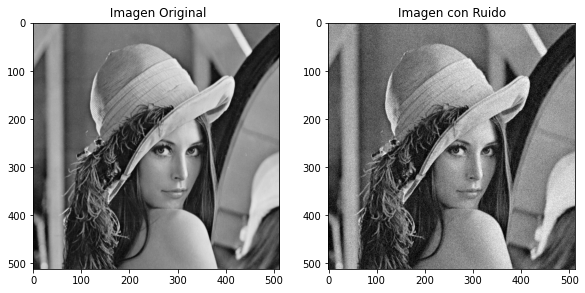
\includegraphics[width=0.7\linewidth]{graficas/lena}
\end{center}

Los parámetros usados para la función objetivo fueron
\begin{center}
	\begin{tabular}{cc}
		\hline
		Parámetro & Valor \\
		\hline
		$n $ & 512 \\
		$ \mu $  & $ 0.01 $ \\
		$ \lambda $ & $ \{ 0.1, 1, 2 \} $ \\
		\hline
	\end{tabular}
\end{center}
Para búsqueda en línea se utilizó
\begin{center}
	\begin{tabular}{cccccc}
		\hline
		Parámetro & $ max_{iter} $ & $ \alpha $ & $ c_1 $ & $ \rho $ & $ \tau_{grad} $ \\
		\hline
		 Valor    &      500     & $ 0.9 $ & $ 10^{-4} $ & $ 0.5 $ &$ 10^{-8} $  \\
		\hline
	\end{tabular}
\end{center}
Dado que siempre se comienza del mismo punto inicial, el experimento sólo se repitió una vez para diferentes valores de $ \lambda $. 
\subsection{Fletcher-Reeves (FR)}
\begin{center}
	\begin{tabular}{rcc}
		\hline
		\hline
		Algoritmo          & Tiempo       & Iteraciones \\
		\hline
		\hline
		$ \lambda = 0.1 $ & 293.75 seg &    1000         \\
		$ \lambda = 1.0 $ & 301.64 seg &    1000         \\
		$ \lambda = 2.0 $ & 322.23 seg &    1000          \\
		\hline
	\end{tabular}
\end{center}
\subsubsection{$ \lambda = 0.1 $}
\begin{center}
	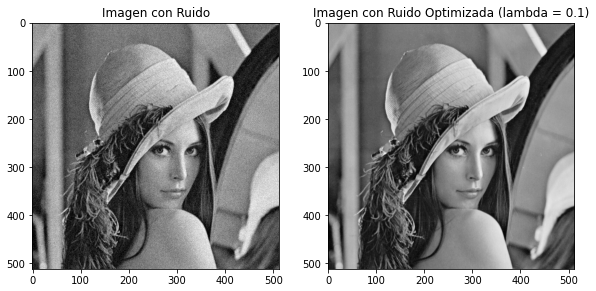
\includegraphics[width=0.75\linewidth]{graficas/fr/optimizada_0}
\end{center}

\begin{center}
	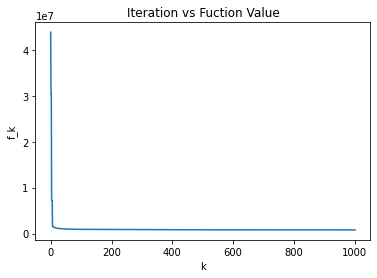
\includegraphics[width=0.6\linewidth]{graficas/fr/funcion_0}
	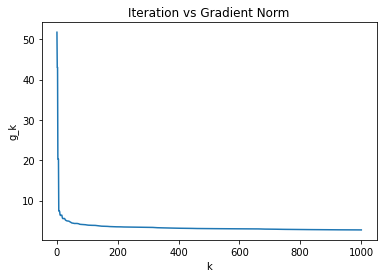
\includegraphics[width=0.6\linewidth]{graficas/fr/gradiente_0}
\end{center}

\subsubsection{$ \lambda = 1 $}
\begin{center}
	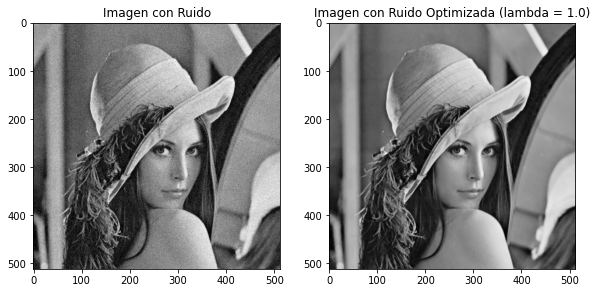
\includegraphics[width=0.7\linewidth]{graficas/fr/optimizada_1}
\end{center}

\begin{center}
	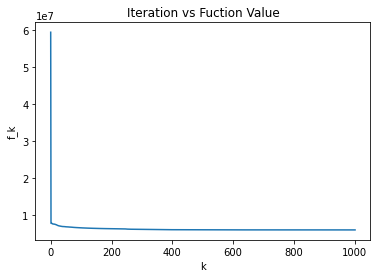
\includegraphics[width=0.6\linewidth]{graficas/fr/funcion_1}
	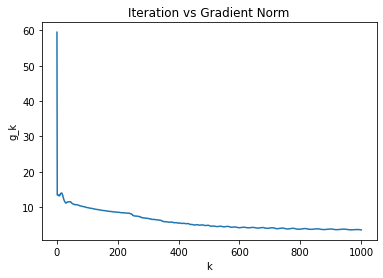
\includegraphics[width=0.6\linewidth]{graficas/fr/gradiente_1}
\end{center}

\subsubsection{$ \lambda = 2 $}
\begin{center}
	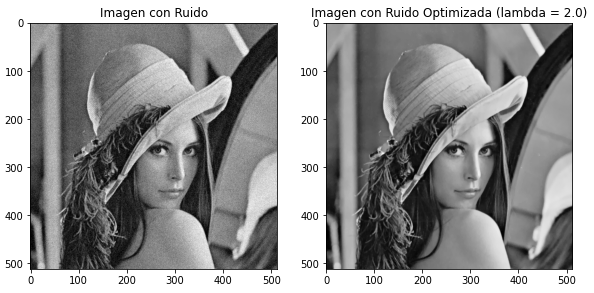
\includegraphics[width=0.7\linewidth]{graficas/fr/optimizada_2}
\end{center}

\begin{center}
	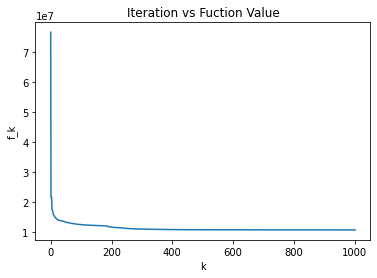
\includegraphics[width=0.6\linewidth]{graficas/fr/funcion_2}
	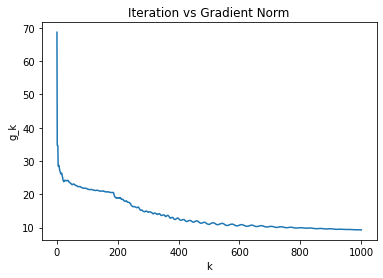
\includegraphics[width=0.6\linewidth]{graficas/fr/gradiente_2}
\end{center}


\subsection{Polak-Ribiere(PR)}
\begin{center}
	\begin{tabular}{rcc}
		\hline
		\hline
		Algoritmo          & Tiempo       & Iteraciones \\
		\hline
		\hline
		$ \lambda = 0.1 $ & 19.10 seg &    60          \\
		$ \lambda = 1.0 $ & 26.30 seg &    92          \\
		$ \lambda = 2.0 $ & 73.80 seg &    256         \\
		\hline
	\end{tabular}
\end{center}
\subsubsection{$ \lambda = 0.1 $}
\begin{center}
	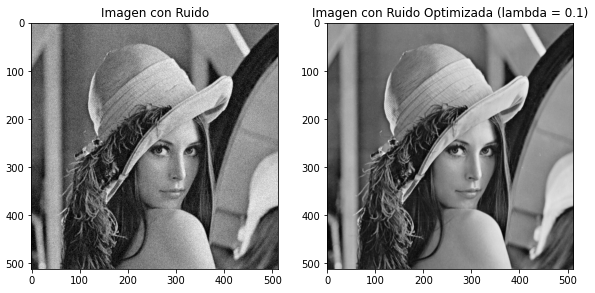
\includegraphics[width=0.75\linewidth]{graficas/pr/optimizada_0}
\end{center}

\begin{center}
	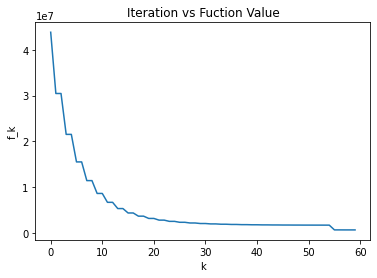
\includegraphics[width=0.6\linewidth]{graficas/pr/funcion_0}
	\includegraphics[width=0.6\linewidth]{graficas/pr/gradiente_0}
\end{center}

\subsubsection{$ \lambda = 1 $}
\begin{center}
	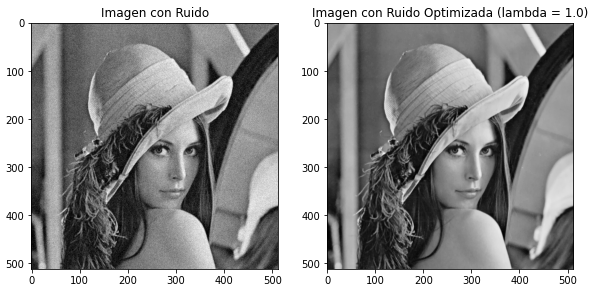
\includegraphics[width=0.7\linewidth]{graficas/pr/optimizada_1}
\end{center}

\begin{center}
	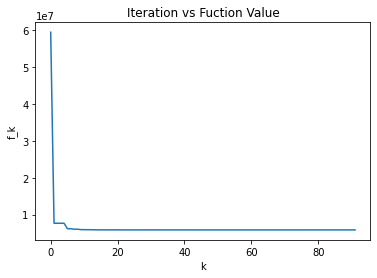
\includegraphics[width=0.6\linewidth]{graficas/pr/funcion_1}
	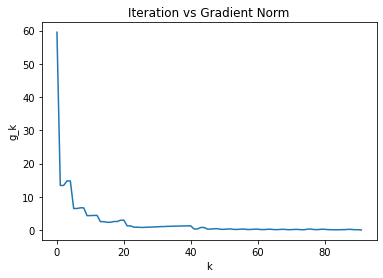
\includegraphics[width=0.6\linewidth]{graficas/pr/gradiente_1}
\end{center}

\subsubsection{$ \lambda = 2 $}
\begin{center}
	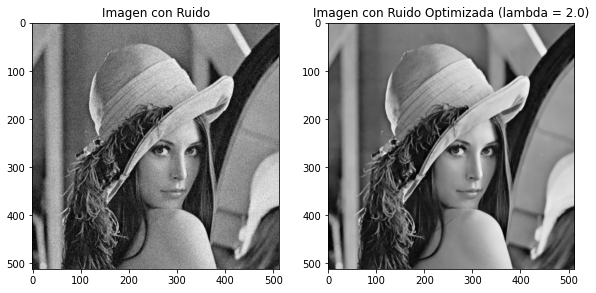
\includegraphics[width=0.75\linewidth]{graficas/pr/optimizada_2}
\end{center}

\begin{center}
	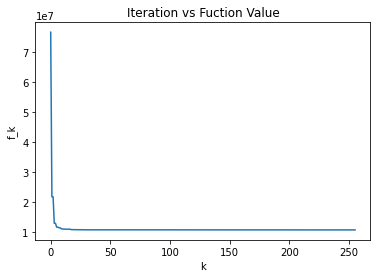
\includegraphics[width=0.6\linewidth]{graficas/pr/funcion_2}
	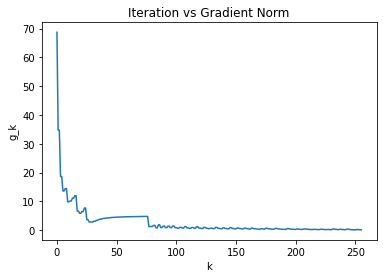
\includegraphics[width=0.6\linewidth]{graficas/pr/gradiente_2}
\end{center}

\subsection{Hestenes-Stiefel (HS)}
\begin{center}
	\begin{tabular}{rcc}
		\hline
		\hline
		Algoritmo          & Tiempo       & Iteraciones \\
		\hline
		\hline
		$ \lambda = 0.1 $ & 9.56 seg &    48          \\
		$ \lambda = 1.0 $ & 20.52 seg &   72          \\
		$ \lambda = 2.0 $ & 38.79 seg &   138         \\
		\hline
	\end{tabular}
\end{center}
\subsubsection{$ \lambda = 0.1 $}
\begin{center}
	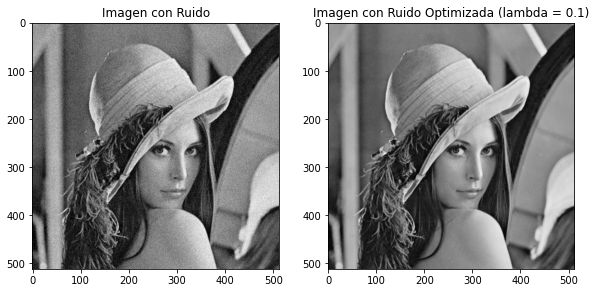
\includegraphics[width=0.75\linewidth]{graficas/hs/optimizada_0}
\end{center}

\begin{center}
	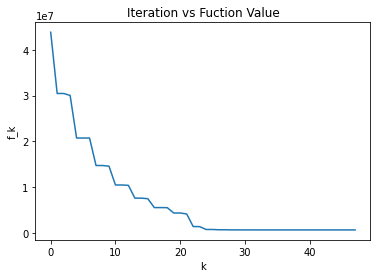
\includegraphics[width=0.6\linewidth]{graficas/hs/funcion_0}
	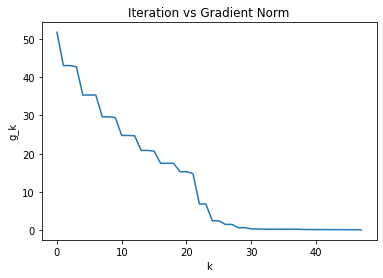
\includegraphics[width=0.6\linewidth]{graficas/hs/gradiente_0}
\end{center}

\subsubsection{$ \lambda = 1 $}
\begin{center}
	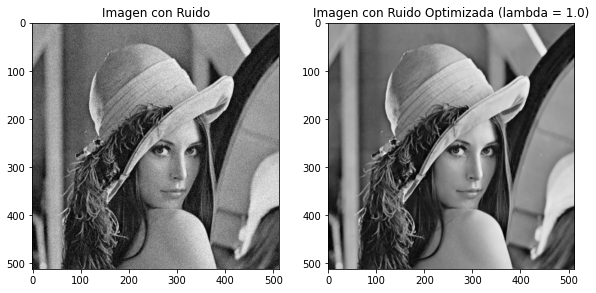
\includegraphics[width=0.75\linewidth]{graficas/hs/optimizada_1}
\end{center}

\begin{center}
	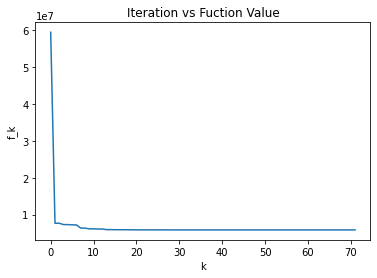
\includegraphics[width=0.6\linewidth]{graficas/hs/funcion_1}
	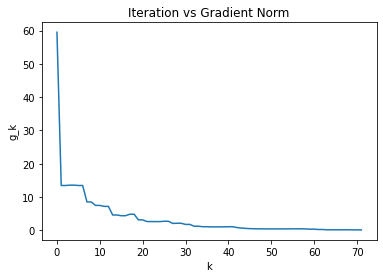
\includegraphics[width=0.6\linewidth]{graficas/hs/gradiente_1}
\end{center}

\subsubsection{$ \lambda = 2 $}
\begin{center}
	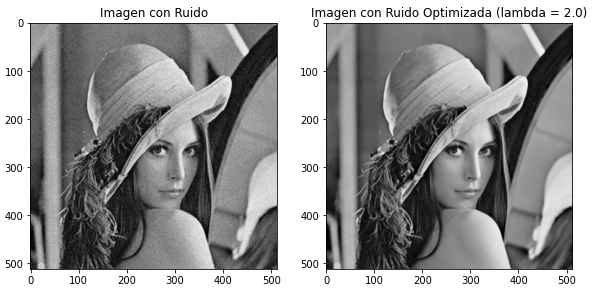
\includegraphics[width=0.75\linewidth]{graficas/hs/optimizada_2}
\end{center}

\begin{center}
	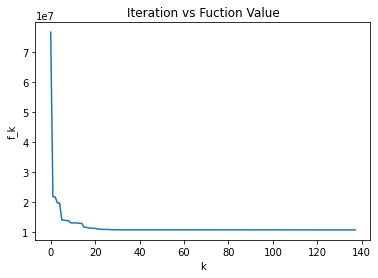
\includegraphics[width=0.6\linewidth]{graficas/hs/funcion_2}
	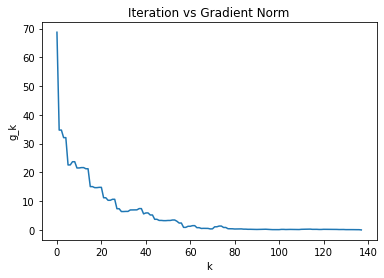
\includegraphics[width=0.6\linewidth]{graficas/hs/gradiente_2}
\end{center}

\subsection{Fletcher-Reeves Polak-Ribiere}
\begin{center}
	\begin{tabular}{rcc}
		\hline
		\hline
		Algoritmo          & Tiempo       & Iteraciones \\
		\hline
		\hline
		$ \lambda = 0.1 $ & 14.19 seg &    60         \\
		$ \lambda = 1.0 $ & 21.85 seg &    88          \\
		$ \lambda = 2.0 $ & 75.19 seg &    277          \\
		\hline
	\end{tabular}
\end{center}
\subsubsection{$ \lambda = 0.1 $}
\begin{center}
	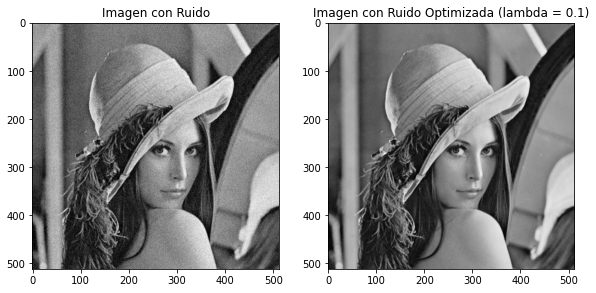
\includegraphics[width=0.75\linewidth]{graficas/frpr/optimizada_0}
\end{center}

\begin{center}
	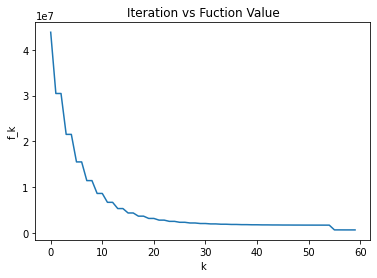
\includegraphics[width=0.6\linewidth]{graficas/frpr/funcion_0}
	\includegraphics[width=0.6\linewidth]{graficas/frpr/gradiente_0}
\end{center}

\subsubsection{$ \lambda = 1 $}
\begin{center}
	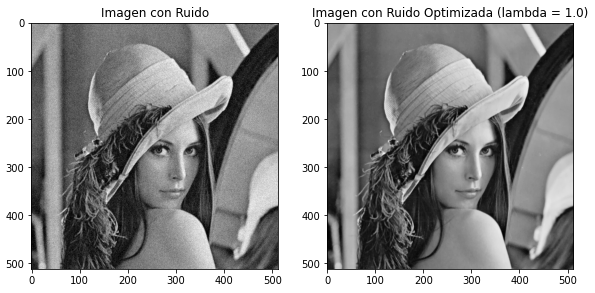
\includegraphics[width=0.75\linewidth]{graficas/frpr/optimizada_1}
\end{center}

\begin{center}
	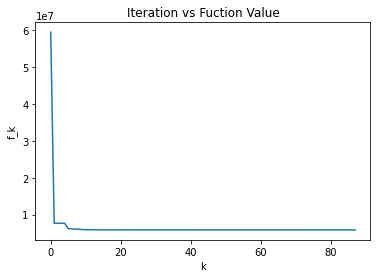
\includegraphics[width=0.6\linewidth]{graficas/frpr/funcion_1}
	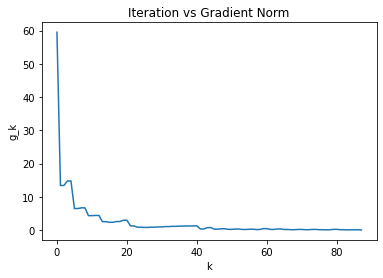
\includegraphics[width=0.6\linewidth]{graficas/frpr/gradiente_1}
\end{center}

\subsubsection{$ \lambda = 2 $}
\begin{center}
	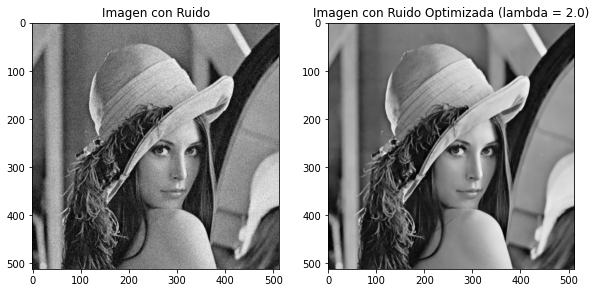
\includegraphics[width=0.75\linewidth]{graficas/frpr/optimizada_2}
\end{center}

\begin{center}
	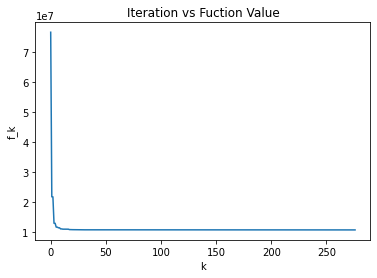
\includegraphics[width=0.6\linewidth]{graficas/frpr/funcion_2}
	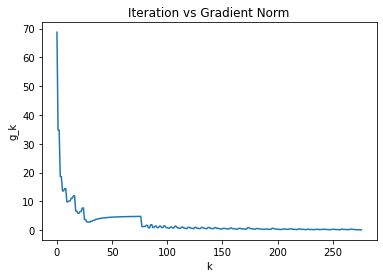
\includegraphics[width=0.6\linewidth]{graficas/frpr/gradiente_2}
\end{center}


\section{Conclusiones}
	En la experimentación se observó que el método de \textbf{Fletcher-Reeves} no convergió para ninguna elección de $ \lambda $. Lo anterior se debe a que dicho algoritmo pide ortogonalidad entre direcciones consecutivas, lo cual no se cumple a priori. A pesar de lo anterior, las imágenes resultantes son parecidas a la imagen original.
	\\
	Para el resto de los métodos se observó una rápida convergencia respecto al número de iteraciones. En primer lugar el método de \textbf{Hestenes-Stiefel} mostró menor número de iteraciones para todas las configuraciones. El método que itera entre \textbf{FR-PR} mejoró respecto al método original \textbf{FR}.
	\\
	Respecto al valor de $ \lambda $, en la experimentación se observó que el algoritmo de \textbf{gradiente conjugado no lineal} mostró un  mejor desempeño para $ \lambda $'s pequeños, i.e, $ \lambda \in (0,1) $. Esto refleja la aportación de los vecinos de un pixel dado para eliminar el ruido. Si $ \lambda $ es grande, i.e, $ \lambda \sim 100 $, el algoritmo elimina más información de la requerida por la imagen original.
\end{document}